\documentclass[bachelor, substylefile=VolSU.rtx]{disser}

\usepackage{placeins}

\usepackage[
  a4paper, mag=1000,
  left=3.0cm, right=1cm, top=2cm, bottom=2cm, headsep=0.7cm, footskip=1cm
]{geometry}

\usepackage[T2A]{fontenc}
\usepackage[utf8]{inputenc}
\usepackage[english, russian]{babel}

\usepackage{amsmath, amssymb, amsfonts}
\usepackage{graphicx, epsfig}
\usepackage{enumitem} 
\numberwithin{equation}{section}


\renewcommand\labelenumi{\theenumi}

\usepackage{listings}
\usepackage{caption3}

\usepackage{makecell}
\usepackage{multirow}
\usepackage{pdflscape}

\usepackage{color}
\def\bEDITS{\global\color{red}}
\def\fEDITS{\global\color{blue}}
\def\eEDITS{\global\color{black}}
\usepackage[colorlinks=false,linkcolor=blue,breaklinks]{hyperref}

% Красным выделены сведения, которые нужно проверить и заполнить по приказу
\newcommand{\fillme}[1]{\textcolor{red}{#1}}

\usepackage[citestyle=gost-numeric,style=gost-numeric,natbib=true,urldate=long, sorting=none,autolang=other]{biblatex}
\usepackage{csquotes}
\pagestyle{footcenter}
\chapterpagestyle{footcenter}

%для борьбы с переполнениями за счет разреженных слов в абзаце
\emergencystretch=5em

\graphicspath{{fig/}}
\addbibresource{Bib.bib}


\usepackage{xcolor}
\definecolor{codegreen}{rgb}{0,0.6,0}
\definecolor{codegray}{rgb}{0.5,0.5,0.5}
\definecolor{codepurple}{rgb}{0.58,0,0.82}
\definecolor{backcolour}{rgb}{0.95,0.95,0.92}
\lstset{extendedchars=\true}
\lstdefinestyle{mystyle}{
    %backgroundcolor=\color{backcolour},
    basicstyle=\ttfamily\normalsize,
    breakatwhitespace=false,         
    breaklines=true,                 
    captionpos=t,                
    keepspaces=true,                 
    numbers=left,                    
    numbersep=5pt,                  
    showspaces=false,                
    showstringspaces=false,
    showtabs=false,                  
    tabsize=2
}
\lstset{style=mystyle}


\RequirePackage{caption}
\DeclareCaptionLabelSeparator{defffis}{ -- }
\captionsetup{justification=centering,labelsep=defffis}

%    \DeclareCaptionLabelSeparator{dottt}{~--- }
%    \captionsetup{labelsep=dottt, font=normalfont}

\begin{document}
\sloppy

\institution{Волгоградский государственный университет \\
Институт математики и информационных технологий \\
Кафедра информационных систем и компьютерного моделирования}

% Название практики и семестр
\title{Отчет по производственной практике, научно-исследовательской работе}
\semester{седьмой семестр}
\topic{Параллельная OpenMP-версия программы для численного моделирования теплопередачи в сплошных средах}

\apname{А. В. Хоперсков}
% Автор (ФИО полностью — требование нормоконтроля)
\author{Богунь Марк Витальевич}
\authorshort{Богунь Марк Витальевич}
% Группа
\group{ПРИб-231}
\coursenum{09.03.04}
\course{Программная инженерия}

% Руководитель практики (ФИО полностью, как в приказе)
\supervisor       {\fillme{Двужилова Ю. В. --- указать ФИО полностью}}
\supervisorstatus {д.ф.-м.н., доцент каф. ИСКМ}
% Организатор практики
\organizer        {С. С. Храпов}
\organizerstatus  {к.ф.-м.н., доцент каф. ИСКМ}

\city{Волгоград}
\date{\number\year}

\maketitle


\renewcommand\contentsname{Содержание}
\tableofcontents

\intro

Численное моделирование теплопередачи широко применяется при проектировании изделий машиностроения, энергетики и электроники, где температурный режим определяет надёжность конструкции~\cite{krainov2016}. Описание процесса строится на уравнении теплопроводности Фурье--Кирхгофа~\cite{chichko2013mathematical}, которое для тел сложной формы и при неоднородных граничных условиях, как правило, не имеет аналитического решения. Поэтому на практике используют сеточные методы, в которых расчётная область заменяется множеством узлов, а производные --- конечными разностями~\cite{kolgan1975finite}.

В предыдущем семестре был разработан программный комплекс HeatSim3D, который решает трёхмерную нестационарную задачу теплопроводности по явной конечно-разностной схеме FTCS. Комплекс состоит из расчётного модуля на языке C++~\cite{stroustrup1986overview} и графического интерфейса на языке Python~\cite{python2021python}. Работа с ним показала, что время расчёта быстро растёт при измельчении сетки. При уменьшении шага сетки вдвое число узлов увеличивается в восемь раз, а допустимый шаг по времени из условия устойчивости уменьшается в четыре раза, так что общий объём вычислений возрастает примерно в тридцать два раза. Для сетки из нескольких миллионов узлов один расчёт в последовательном режиме занимает уже минуты, а серия расчётов для разных материалов и граничных условий --- часы.

Современные персональные компьютеры оснащены многоядерными процессорами, однако последовательная программа использует только одно ядро. Наиболее простой способ задействовать все ядра в программе на C++ даёт технология OpenMP~\cite{dagum1998openmp}, которая позволяет распараллелить существующий код добавлением директив компилятора без изменения структуры алгоритма~\cite{chandra2001parallel}. При этом важно не только получить выигрыш во времени, но и доказать, что параллельная программа выдаёт те же результаты, что и последовательная, а также оценить, насколько полно используются вычислительные ресурсы. Именно количественная оценка ускорения и анализ факторов, которые его ограничивают, составляют исследовательскую часть работы.

Целью работы является разработка и исследование параллельной OpenMP-версии программного комплекса HeatSim3D для численного моделирования нестационарной теплопередачи в сплошных средах.

Для достижения поставленной цели необходимо решить следующие задачи:
\begin{enumerate}[label=\arabic*.]
    \item Изучить технологию OpenMP и показатели эффективности параллельных программ для систем с общей памятью.
    \item Проанализировать информационные зависимости алгоритма явной схемы FTCS и выделить участки, допускающие параллельное выполнение.
    \item Разработать параллельную версию расчётного модуля с управляемым числом потоков, совместимую с компиляторами GCC, MinGW и Microsoft Visual C++.
    \item Обеспечить сборку и работу программного комплекса в операционных системах Linux и Windows.
    \item Проверить корректность параллельной версии путём сравнения с аналитическим решением и с результатами последовательного расчёта.
    \item Исследовать ускорение и эффективность параллельной версии для расчётных сеток разного размера и оценить влияние последовательной записи результатов.
\end{enumerate}

Новизна работы для программного комплекса HeatSim3D состоит в том, что параллельный режим впервые снабжён средствами управления числом потоков и автоматического замера производительности. Это позволило перейти от качественного утверждения об ускорении расчёта к измеренным значениям ускорения и эффективности. Кроме того, разработан модуль построения графиков в оформлении, пригодном для научного отчёта, и набор автоматических тестов, подтверждающих корректность параллельной версии.

В первой главе приводится краткое описание математической модели и численного метода, рассматриваются модель исполнения OpenMP и показатели эффективности параллельных программ. Во второй главе описана разработка параллельной версии расчётного модуля, включая анализ зависимостей по данным, выбор директив OpenMP и обеспечение кроссплатформенности. В третьей главе представлены результаты проверки корректности и исследования производительности параллельной версии на многоядерном процессоре.

\chapter{Параллельные вычисления в задаче моделирования теплопередачи}

\section{Математическая модель нестационарной теплопроводности в трёхмерной области}

\subsection{Уравнение теплопроводности с граничными условиями первого рода}

Рассматривается однородное изотропное твёрдое тело в форме куба $\Omega = [0, L]^3$ с длиной ребра $L = 1$~м. Распределение температуры $T(x, y, z, t)$ в нём при отсутствии внутренних источников тепла описывается уравнением теплопроводности Фурье--Кирхгофа~\cite{сергиенко2004исследование}
\begin{equation}
    \frac{\partial T}{\partial t} = a \left( \frac{\partial^2 T}{\partial x^2} + \frac{\partial^2 T}{\partial y^2} + \frac{\partial^2 T}{\partial z^2} \right),
    \label{eq:heat}
\end{equation}
где $a$ --- коэффициент температуропроводности материала, м$^2$/с. Этот коэффициент равен отношению теплопроводности к произведению плотности на удельную теплоёмкость и характеризует скорость выравнивания температуры в теле~\cite{vlasov2004research}. Для конструкционной стали, которая используется в расчётах данной работы, принято значение $a = 1{,}28 \cdot 10^{-5}$~м$^2$/с.

Для однозначного решения уравнения~\eqref{eq:heat} задаются начальное и граничные условия~\cite{luo2010effect}. В начальный момент температура во всех точках тела одинакова и равна $T_0$. На каждой из шести граней куба поддерживается собственная постоянная температура, то есть используются граничные условия первого рода, или условия Дирихле~\cite{дирихлерешении}. Например, на гранях, перпендикулярных оси $x$, они имеют вид
\begin{equation}
    T\big|_{x=0} = T_{x-}, \qquad T\big|_{x=L} = T_{x+},
\end{equation}
а на остальных гранях записываются аналогично. Независимое задание температуры на каждой грани позволяет моделировать как равномерный прогрев тела, так и направленный тепловой поток. Подробный вывод уравнения и обсуждение физического смысла его параметров приведены в отчёте за предыдущий семестр, поэтому здесь математическая модель изложена кратко.

\subsection{Явная конечно-разностная схема и условие её устойчивости}

Расчётная область покрывается равномерной сеткой из $N_x \times N_y \times N_z$ узлов с шагами $h_x = L / (N_x - 1)$, $h_y$ и $h_z$, которые определяются аналогично. Обозначим через $T^n_{i,j,k}$ приближённое значение температуры в узле с индексами $(i, j, k)$ в момент времени $t_n = n \Delta t$. Замена производной по времени разностью вперёд, а вторых производных по пространству центральными разностями приводит к явной схеме FTCS~\cite{kolgan1975finite}
\begin{equation}
    T^{n+1}_{i,j,k} = T^n_{i,j,k} + r_x \, \delta_x^2 T^n_{i,j,k} + r_y \, \delta_y^2 T^n_{i,j,k} + r_z \, \delta_z^2 T^n_{i,j,k},
    \label{eq:ftcs}
\end{equation}
в которой использованы обозначения $\delta_x^2 T_{i,j,k} = T_{i+1,j,k} - 2T_{i,j,k} + T_{i-1,j,k}$ и $r_x = a \Delta t / h_x^2$, а величины для осей $y$ и $z$ определяются так же. Схема~\eqref{eq:ftcs} имеет первый порядок аппроксимации по времени и второй порядок по пространству.

Явная схема устойчива только при ограничении на шаг по времени~\cite{dubey2015stability}. Для трёхмерной задачи оно записывается в виде неравенства
\begin{equation}
    2 \left( r_x + r_y + r_z \right) \le 1,
    \label{eq:stab}
\end{equation}
поэтому в программе шаг $\Delta t$ выбирается автоматически так, чтобы левая часть~\eqref{eq:stab} равнялась 0,4. Такой запас исключает рост ошибок округления при любых допустимых параметрах расчёта. Из неравенства~\eqref{eq:stab} следует, что шаг по времени пропорционален квадрату шага сетки, и именно это делает расчёт на мелких сетках трудоёмким.

Для дальнейшего важно одно свойство схемы~\eqref{eq:ftcs}. Новое значение температуры в узле вычисляется только по значениям с предыдущего временного слоя в самом узле и в шести соседних узлах. Следовательно, на одном шаге по времени все внутренние узлы можно обрабатывать независимо друг от друга и в произвольном порядке, что и создаёт возможность для параллельных вычислений.

\section{Технология OpenMP для вычислительных систем с общей памятью}

\subsection{Модель исполнения fork--join и директивы распараллеливания циклов}

OpenMP представляет собой стандарт программного интерфейса для параллельного программирования на языках C, C++ и Fortran в системах с общей памятью~\cite{dagum1998openmp}. Стандарт включает директивы компилятора, библиотечные функции и переменные окружения\footnote{Актуальные версии спецификации OpenMP публикуются на официальном сайте OpenMP Architecture Review Board: \url{https://www.openmp.org}.}. Программа начинает работу в одном главном потоке, а при входе в параллельную область создаётся группа потоков, которые выполняют её совместно. По завершении области потоки синхронизируются, и выполнение продолжается в главном потоке. Такая схема называется моделью fork--join~\cite{chandra2001parallel}.

В вычислительных программах основная работа сосредоточена в циклах, поэтому наиболее употребительна директива \texttt{parallel for}. Она распределяет итерации следующего за ней цикла между потоками группы, причём программисту не требуется вручную создавать потоки и делить диапазон индексов~\cite{antonov2009openmp}. Все потоки работают в общем адресном пространстве, поэтому массивы доступны каждому из них без копирования. Обратной стороной общей памяти является риск гонки данных, при которой несколько потоков одновременно изменяют одну и ту же ячейку и результат зависит от порядка их выполнения. Если программа компилируется без поддержки OpenMP, директивы игнорируются и получается обычная последовательная программа, что удобно для сравнения двух версий.

\subsection{Распределение итераций между потоками и редукция данных}

Способ распределения итераций задаётся параметром \texttt{schedule}. При статическом распределении диапазон итераций заранее делится на равные непрерывные части по числу потоков, а при динамическом распределении потоки получают новые порции итераций по мере завершения предыдущих~\cite{antonov2009openmp}. Статическое распределение не требует дополнительной синхронизации во время работы цикла и поэтому предпочтительно, когда все итерации выполняют одинаковый объём вычислений. Для вложенных циклов стандарт, начиная с версии 3.0, предоставляет параметр \texttt{collapse}, объединяющий несколько циклов в одно пространство итераций.

Отдельного внимания требуют циклы, в которых все итерации накапливают результат в одной переменной, например при суммировании элементов массива. Параметр \texttt{reduction} создаёт для каждого потока собственную копию такой переменной, а по окончании цикла объединяет частичные результаты~\cite{chandra2001parallel}. Этот приём устраняет гонку данных без использования блокировок. Однако порядок сложения при этом меняется, и для чисел с плавающей точкой результат может отличаться от последовательного в последних значащих разрядах.

\section{Показатели эффективности параллельных программ и их ограничения}

\subsection{Ускорение и эффективность параллельной программы на многоядерном процессоре}

Качество распараллеливания оценивается по времени выполнения одной и той же задачи на разном числе потоков. Если $t_1$ --- время расчёта одним потоком, а $t_p$ --- время расчёта $p$ потоками, то ускорение и эффективность определяются выражениями
\begin{equation}
    S_p = \frac{t_1}{t_p}, \qquad E_p = \frac{S_p}{p}.
    \label{eq:speedup}
\end{equation}
В идеальном случае ускорение равно числу потоков, а эффективность равна единице. На практике эффективность меньше единицы из-за затрат на создание и синхронизацию потоков, неравномерной загрузки и наличия участков программы, которые выполняются последовательно. Значения эффективности выше 0,8 обычно считаются хорошим результатом для программ с общей памятью.

\subsection{Закон Амдала и ограничение пропускной способностью памяти}

Пусть доля $f$ времени работы последовательной программы приходится на участки, которые не распараллеливаются. Тогда по закону Амдала~\cite{amdahl1967validity} ускорение на $p$ потоках не может превысить величину
\begin{equation}
    S_p = \frac{1}{f + (1 - f)/p},
    \label{eq:amdahl}
\end{equation}
и при неограниченном увеличении числа потоков стремится к $1/f$. Например, при $f = 0{,}1$ ускорение на четырёх потоках не превышает 3,1, а на любом числе потоков --- 10. В программе моделирования теплопередачи последовательной частью является прежде всего запись промежуточных результатов в файлы, поскольку она выполняется одним потоком.

Второе ограничение связано с работой памяти. При вычислении нового значения по формуле~\eqref{eq:ftcs} на каждый узел приходится около десяти арифметических операций и обращение к семи значениям массива. Процессор выполняет такие операции быстрее, чем память успевает доставлять данные, поэтому скорость расчёта определяется пропускной способностью памяти. Ядра процессора разделяют общую шину памяти и кэш последнего уровня~\cite{кудухов2014особенности}, и с ростом числа потоков каждое ядро получает меньшую долю этой пропускной способности. По этой причине для задач со стенсильными вычислениями эффективность обычно снижается с ростом числа потоков даже при отсутствии последовательных участков.

\chapter{Разработка параллельной OpenMP-версии программного комплекса HeatSim3D}

\section{Анализ информационных зависимостей вычислительного алгоритма схемы FTCS}

\subsection{Независимость вычислений во внутренних узлах на одном шаге}

Расчётный модуль HeatSim3D принимает параметры задачи через аргументы командной строки, выполняет цикл по времени и сохраняет результаты в файлы формата CSV. Каждый шаг по времени состоит из трёх действий. Сначала по формуле~\eqref{eq:ftcs} вычисляются новые значения во всех внутренних узлах, затем на шести гранях восстанавливаются граничные значения, и, наконец, с заданной периодичностью в файлы записываются срезы поля и температура в центре тела.

Первое действие занимает основную часть времени расчёта, так как число внутренних узлов равно $(N_x - 2)(N_y - 2)(N_z - 2)$ и для сетки $150^3$ превышает три миллиона. Как отмечено в первой главе, значение в каждом узле нового слоя зависит только от значений предыдущего слоя. Поэтому между итерациями цикла по внутренним узлам отсутствуют зависимости по данным, и цикл может выполняться параллельно без изменения результата. Между шагами по времени, напротив, существует строгая зависимость, поскольку следующий шаг использует результат предыдущего. Таким образом, распараллеливанию подлежит обработка узлов внутри шага, а сам цикл по времени остаётся последовательным.

\subsection{Организация двух буферов температурного поля в памяти}

Температурное поле хранится в одномерном массиве \texttt{std::vector<double>} длиной $N_x N_y N_z$, а узлу с индексами $(i, j, k)$ соответствует элемент с номером $i N_y N_z + j N_z + k$. При такой нумерации соседние по индексу $k$ узлы расположены в памяти подряд, что позволяет процессору эффективно использовать кэш при последовательном проходе по внутреннему циклу.

Для корректной параллельной работы используются два массива одинакового размера. Первый массив содержит значения на текущем слое и во время шага только читается, а во второй массив записываются новые значения. После завершения шага массивы меняются ролями с помощью функции \texttt{std::swap}, которая обменивает внутренние указатели и не копирует данные. При такой организации каждый элемент нового массива записывается ровно одним потоком, а читаемый массив не изменяется, поэтому гонка данных невозможна. Синхронизация требуется только перед обменом массивов, и её обеспечивает неявный барьер в конце директивы \texttt{parallel for}.

\section{Распараллеливание основных вычислительных циклов расчётного модуля}

\subsection{Слияние пространственных циклов для равномерной загрузки потоков}

В исходной версии программы цикл по внутренним узлам состоял из трёх вложенных циклов по индексам $i$, $j$ и $k$. Если распараллелить только внешний цикл, то число его итераций $N_x - 2$ при небольших сетках сравнимо с числом потоков, и часть потоков может получить на одну итерацию больше других. В версии прошлого семестра для объединения двух внешних циклов использовался параметр \texttt{collapse(2)}. Однако этот параметр появился только в стандарте OpenMP 3.0, а компилятор Microsoft Visual C++ с ключом \texttt{/openmp} поддерживает стандарт 2.0, и программа в этой среде не собиралась бы.

Поэтому в новой версии слияние циклов выполнено вручную. Вводится единый индекс $m$, пробегающий значения от 0 до $(N_x - 2)(N_y - 2) - 1$, а исходные индексы восстанавливаются по формулам
\begin{equation}
    i = 1 + \left\lfloor \frac{m}{N_y - 2} \right\rfloor, \qquad j = 1 + m \bmod (N_y - 2),
\end{equation}
после чего внутри итерации последовательно обрабатывается весь столбец узлов по индексу $k$. Директива \texttt{parallel for} со статическим распределением применяется к циклу по $m$. Уже для сетки $50^3$ число итераций равно 2304, поэтому части, достающиеся потокам, практически одинаковы. Внутренний цикл по $k$ проходит по памяти подряд и хорошо оптимизируется компилятором.

\subsection{Параллельное наложение граничных условий и вычисление средней температуры}

Наложение граничных условий выполняется после каждого шага и состоит из трёх пар циклов, каждая из которых заполняет две противоположные грани куба. Объём этой работы пропорционален $N^2$, а не $N^3$, однако при последовательном выполнении она превращалась бы в постоянную последовательную долю каждого шага. Поэтому каждая пара циклов также снабжена директивой \texttt{parallel for}. Записи в разные элементы массива не пересекаются, и синхронизация внутри этих циклов не нужна.

При каждой записи результатов программа вычисляет среднюю температуру по объёму тела, то есть сумму значений во всех узлах. Для этого цикла использована редукция \texttt{reduction(+:sum)}, при которой каждый поток суммирует свою часть массива, а частичные суммы объединяются по окончании цикла~\cite{chandra2001parallel}. Из-за изменения порядка сложения средняя температура может отличаться от последовательного значения на величину порядка $10^{-13}$~°C. Такое отличие не проявляется в файлах результатов, где значения записываются с четырьмя знаками после запятой.

\subsection{Управление числом потоков и измерение времени расчёта}

Для исследования производительности в расчётный модуль добавлен параметр командной строки \texttt{--threads}, который вызывает функцию \texttt{omp\_set\_num\_threads}. Если параметр не указан, используется число потоков, выбранное средой OpenMP по умолчанию, обычно равное числу ядер процессора. Фактическое число потоков выводится в заголовке протокола расчёта и сохраняется вместе со всеми параметрами задачи в файл \texttt{params.csv}. Это позволяет по файлам результатов однозначно установить, в каком режиме был выполнен расчёт.

Время расчёта измеряется средствами библиотеки \texttt{std::chrono} от начала до конца цикла по времени, поэтому выделение памяти и разбор параметров в него не входят. Измеренное время выводится по окончании расчёта и также записывается в \texttt{params.csv}. При сборке без поддержки OpenMP получается последовательная версия программы, в которой параметр \texttt{--threads} не действует, а в протоколе указывается один поток.

\section{Обеспечение кроссплатформенности программного комплекса для Linux и Windows}

\subsection{Сборка расчётного модуля различными компиляторами с поддержкой OpenMP}

Исходный код расчётного модуля написан на стандартном языке C++17 и содержит единственный платформенно-зависимый фрагмент, связанный с созданием каталога для результатов. В операционной системе Windows для этого используется функция \texttt{\_mkdir}, а в Linux --- функция \texttt{mkdir}, и выбор между ними выполняется директивами условной компиляции. Обращения к библиотеке OpenMP также помещены в блоки условной компиляции, поэтому один и тот же файл собирается как в параллельном, так и в последовательном режиме.

Для Linux расчётный модуль собирается компилятором GCC с ключом \texttt{-fopenmp}. Для Windows исполняемый файл получен кросс-компилятором MinGW-w64 на основе GCC 13 со статической компоновкой, благодаря чему он не требует установки дополнительных библиотек на компьютере пользователя. Сборка в среде Microsoft Visual C++ также возможна после включения поддержки OpenMP в свойствах проекта. Графический интерфейс автоматически выбирает исполняемый файл расчётного модуля в зависимости от операционной системы, а для обеих систем подготовлены сценарии сборки, которые также упаковывают интерфейс в один исполняемый файл.

\subsection{Средства построения графиков и автоматизации вычислительных экспериментов}

Для подготовки результатов к отчёту разработан модуль \texttt{report\_plots.py} на языке Python, использующий библиотеку matplotlib~\cite{bisong2019matplotlib}. Модуль строит графики в едином оформлении, в котором кривые различаются типом линии и маркерами, а шрифт на рисунках совпадает со шрифтом основного текста по начертанию и размеру. Помимо графиков динамики температуры и профилей, модуль вычисляет аналитическое решение для проверки модели и выполняет серию запусков расчётного модуля с разным числом потоков для оценки ускорения.

Все вычислительные эксперименты, результаты которых приведены в третьей главе, выполняются одним сценарием \texttt{experiments.py}. Сценарий запускает расчёты, сохраняет исходные данные замеров в файлы CSV и строит по ним рисунки. Такая организация делает результаты воспроизводимыми, поскольку любой рисунок отчёта можно получить повторно на другом компьютере одной командой. Корректность параллельной версии дополнительно контролируется набором автоматических тестов на основе библиотеки pytest, которые проверяют совпадение результатов при разном числе потоков, работу параметра \texttt{--threads} и соответствие аналитическому решению.

\chapter{Вычислительные эксперименты с параллельной версией программного комплекса}

\section{Проверка корректности результатов параллельной версии программы}

\subsection{Сравнение численного решения с аналитическим решением задачи}

Корректность численной модели проверялась на задаче, для которой известно точное решение. Рассматривался прогрев стального куба с начальной температурой $T_0 = 20$~°C, на всех гранях которого поддерживается температура $T_b = 100$~°C. Методом разделения переменных решение такой задачи представляется рядом Фурье, и в центре куба оно принимает вид
\begin{equation}
    T_c(t) = T_b + (T_0 - T_b) \, \frac{64}{\pi^3} \left( \sum_{k = 1, 3, 5, \ldots} \frac{(-1)^{(k-1)/2}}{k} \, e^{-a \pi^2 k^2 t / L^2} \right)^{3},
    \label{eq:analytic}
\end{equation}
где суммирование выполняется по нечётным значениям $k$. Ряд в выражении~\eqref{eq:analytic} распадается на произведение трёх одинаковых одномерных рядов, поэтому его легко вычислить с высокой точностью. В расчётах использовались первые двадцать нечётных членов ряда, чего достаточно при $t > 0$. Численный расчёт выполнялся параллельной версией программы на сетке $31^3$ с шагом по времени 5,79~с до момента $t = 20\,000$~с.

На рисунке~\ref{fig:validation} показано изменение температуры в центре куба, полученное численно и по формуле~\eqref{eq:analytic}, а также модуль их разности. Кривые на рисунке~\ref{fig:validation},~а практически совпадают на всём интервале времени: после короткого начального периода, пока тепло от граней ещё не дошло до центра, температура быстро растёт и затем асимптотически приближается к 100~°C. График погрешности на рисунке~\ref{fig:validation},~б имеет один максимум, равный 0,20~°C, который достигается примерно через 0,55~ч после начала прогрева, когда температура меняется быстрее всего. Это значение составляет 0,25~\% от полного перепада температур 80~°C. По мере выхода на установившийся режим погрешность уменьшается и стремится к нулю, что соответствует поведению устойчивой разностной схемы.

\begin{figure}[ht]
    \centering
    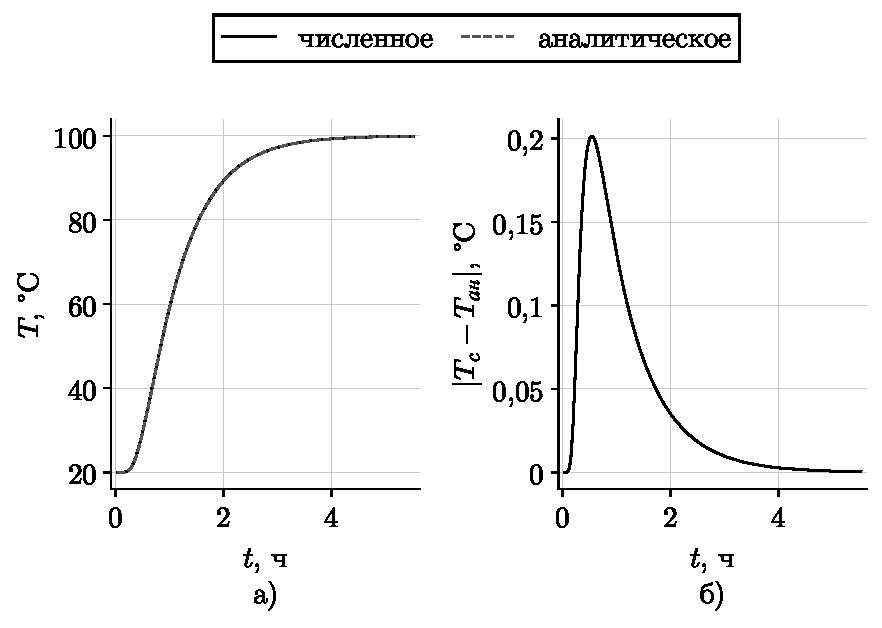
\includegraphics{validation.pdf}
    \caption{Температура в центре куба: численное и аналитическое решения~(а) и абсолютная погрешность численного решения~(б)}
    \label{fig:validation}
\end{figure}

\subsection{Исследование сходимости численного решения при измельчении сетки}

Совпадение с аналитическим решением на одной сетке ещё не доказывает правильность реализации, поскольку ошибка в программе могла бы проявиться только в порядке сходимости. Поэтому расчёт той же задачи был повторён на четырёх сетках, шаг которых последовательно уменьшался вдвое. Шаг по времени при этом выбирался программой автоматически из условия~\eqref{eq:stab}. Погрешность сравнивалась в момент $t = 4000$~с, а численное значение в этот момент находилось линейной интерполяцией между ближайшими шагами по времени. Результаты сравнения приведены в таблице~\ref{tab:conv}.

\begin{table}[ht]
    \centering
    \caption{Погрешность температуры в центре куба при $t = 4000$~с}
    \label{tab:conv}
    \begin{tabular}{|c|c|c|c|c|}
        \hline
        Сетка & $h$, м & $T_c$, °C & $|T_c - T_{\text{ан}}|$, °C & Отношение погрешностей \\
        \hline
        $11^3$ & 0,1000 & 65,383 & 1,0113 & --- \\
        $21^3$ & 0,0500 & 64,626 & 0,2543 & 3,98 \\
        $41^3$ & 0,0250 & 64,435 & 0,0636 & 4,00 \\
        $81^3$ & 0,0125 & 64,387 & 0,0159 & 4,00 \\
        \hline
    \end{tabular}
\end{table}

Аналитическое значение температуры в этот момент равно 64,371~°C. Из таблицы видно, что при каждом уменьшении шага сетки вдвое погрешность уменьшается ровно в четыре раза. Такое поведение означает второй порядок сходимости по пространству, который и должна обеспечивать схема~\eqref{eq:ftcs}. Первый порядок аппроксимации по времени не нарушает эту картину, так как шаг по времени пропорционален $h^2$ и вносимая им ошибка убывает так же быстро.

\subsection{Совпадение результатов при различном числе вычислительных потоков}

Для параллельной программы недостаточно проверить точность одного расчёта, так как ошибки синхронизации проявляются случайно и зависят от числа потоков. Поэтому одна и та же задача с несимметричными граничными условиями на сетке $21^3$ рассчитывалась одним и четырьмя потоками, после чего все файлы результатов сравнивались поэлементно. Значения температуры во всех срезах поля совпали побитно, то есть без какого-либо различия даже в последнем разряде. Такой результат объясняется тем, что каждый узел вычисляется по одной и той же формуле с одними и теми же исходными данными, а от числа потоков зависит только то, какой поток выполняет вычисление.

Аналогичное сравнение было выполнено для исполняемых файлов, собранных для Linux и для Windows. Версия для Windows запускалась в среде совместимости Wine, и её результаты также совпали с результатами версии для Linux побитно, а различие файлов состояло лишь в символах перевода строки. Оба сравнения включены в набор автоматических тестов и выполняются при каждом изменении исходного кода.

\section{Исследование производительности параллельной версии на многоядерном процессоре}

\subsection{Методика проведения замеров времени выполнения расчёта}

Замеры выполнялись на четырёхъядерном процессоре Intel Xeon с тактовой частотой 2,1~ГГц под управлением операционной системы Linux. Расчётный модуль был собран компилятором GCC версии 13.3 с уровнем оптимизации \texttt{-O2}. Рассматривались кубические сетки $50^3$, $100^3$ и $150^3$, содержащие от 125 тысяч до 3,4 миллиона узлов, а число потоков менялось от одного до четырёх.

Чтобы время расчёта на разных сетках было сопоставимым, на каждой сетке выполнялась ровно тысяча шагов по времени, а запись промежуточных результатов была отключена. Каждый расчёт повторялся пять раз, и в качестве результата принималось наименьшее время. Такой выбор исключает случайные задержки, вызванные другими процессами операционной системы, и характеризует возможности самой программы. Ускорение и эффективность вычислялись по формулам~\eqref{eq:speedup}.

\subsection{Ускорение и эффективность для расчётных сеток разного размера}

Измеренное время расчёта приведено в таблице~\ref{tab:bench}. Последовательная версия программы, собранная без поддержки OpenMP, на сетке $100^3$ выполняет расчёт за 2,02~с, то есть практически за то же время, что и параллельная версия на одном потоке. Это означает, что сами директивы OpenMP не создают заметных накладных расходов.

\begin{table}[ht]
    \centering
    \caption{Время расчёта 1000 шагов по времени, с}
    \label{tab:bench}
    \begin{tabular}{|c|c|c|c|c|c|c|}
        \hline
        Сетка & $p = 1$ & $p = 2$ & $p = 3$ & $p = 4$ & $S_4$ & $E_4$ \\
        \hline
        $50^3$  & 0,231 & 0,132 & 0,107 & 0,085 & 2,72 & 0,68 \\
        $100^3$ & 1,879 & 1,010 & 0,737 & 0,548 & 3,43 & 0,86 \\
        $150^3$ & 6,837 & 3,520 & 2,565 & 2,121 & 3,22 & 0,81 \\
        \hline
    \end{tabular}
\end{table}

Зависимость ускорения и эффективности от числа потоков для трёх сеток показана на рисунке~\ref{fig:speedup}. На рисунке~\ref{fig:speedup},~а кривые для сеток $100^3$ и $150^3$ идут вблизи идеальной прямой $S_p = p$ и при четырёх потоках достигают значений 3,43 и 3,22 соответственно. Кривая для сетки $50^3$ заметно отклоняется от идеальной уже при трёх потоках, и итоговое ускорение составляет 2,72. На рисунке~\ref{fig:speedup},~б эта разница видна ещё отчётливее: эффективность для больших сеток при четырёх потоках остаётся на уровне 0,81--0,86, тогда как для малой сетки она снижается до 0,68.

\begin{figure}[ht]
    \centering
    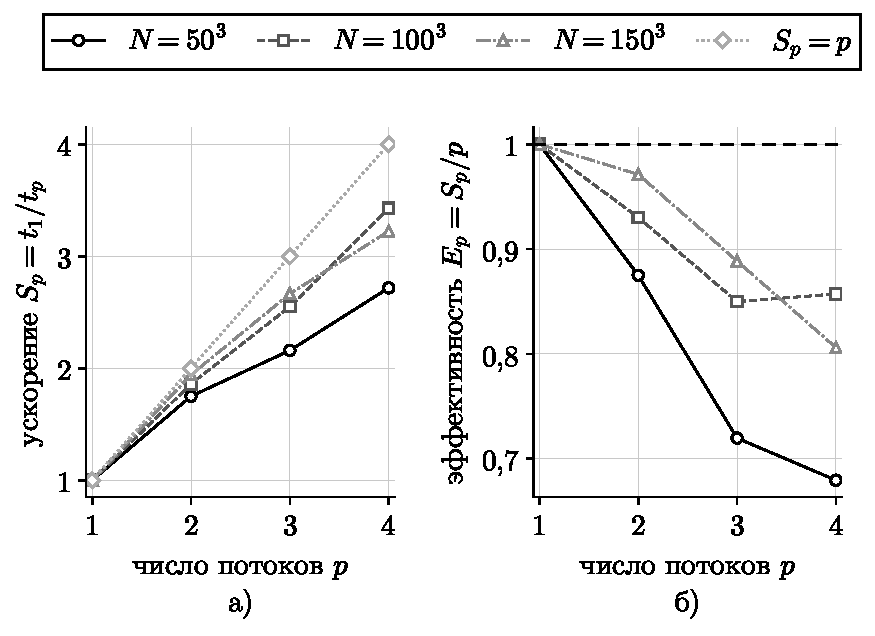
\includegraphics{fig_speedup.pdf}
    \caption{Ускорение~(а) и эффективность~(б) параллельной версии программы в зависимости от числа потоков для сеток разного размера}
    \label{fig:speedup}
\end{figure}

Снижение эффективности на малой сетке объясняется соотношением полезной работы и накладных расходов. На сетке $50^3$ один шаг по времени выполняется за доли миллисекунды, а на каждом шаге программа проходит через четыре параллельные области, в конце каждой из которых потоки синхронизируются. Время синхронизации от размера сетки не зависит, поэтому на малой сетке его доля оказывается значительной. На больших сетках доля синхронизации мала, и основным ограничением становится пропускная способность памяти, о которой говорилось в первой главе. Различие между сетками $100^3$ и $150^3$ находится в пределах разброса повторных замеров, составляющего около 5--10~\%.

\subsection{Влияние последовательной записи результатов на итоговое ускорение}

В рассмотренных замерах запись результатов была отключена, однако в реальной работе программа периодически сохраняет срезы температурного поля для последующей визуализации. Запись в файлы выполняется одним потоком, и для оценки её влияния был проведён отдельный эксперимент на сетке $100^3$. При одной и той же тысяче шагов число записей $M$ менялось от нуля до ста, а время расчёта измерялось на одном и на четырёх потоках. Для сравнения с замерами использовалась простая модель, в которой время записи не уменьшается при увеличении числа потоков, а время вычислений уменьшается так же, как в расчёте без записи.

Результаты эксперимента приведены на рисунке~\ref{fig:io}. На рисунке~\ref{fig:io},~а время расчёта на обоих потоках растёт с увеличением числа записей, причём для одного потока каждая запись добавляет около 17~мс. Поскольку это время одинаково для любого числа потоков, разрыв между кривыми в относительном выражении сокращается. На рисунке~\ref{fig:io},~б видно, что ускорение на четырёх потоках падает с 3,39 при отсутствии записи до 2,16 при двадцати записях и до 1,34 при ста записях.

\begin{figure}[ht]
    \centering
    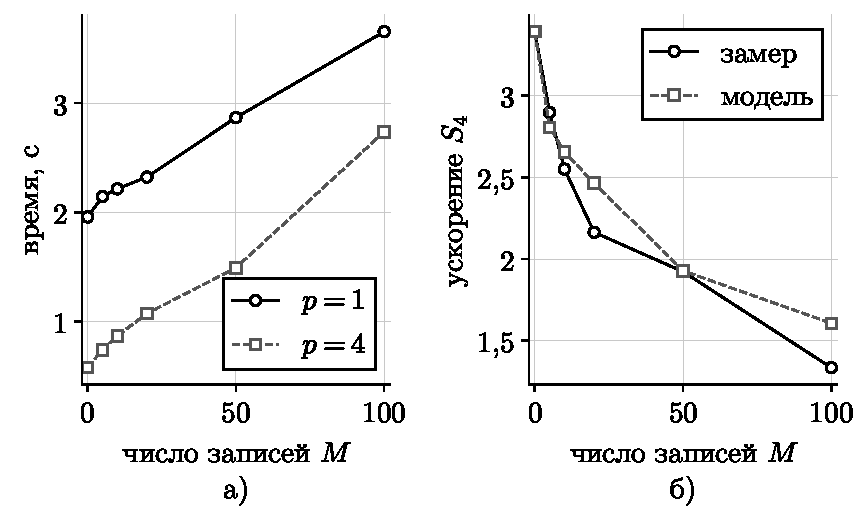
\includegraphics{io.pdf}
    \caption{Время расчёта~(а) и ускорение на четырёх потоках~(б) в зависимости от числа записей результатов на сетке $100^3$}
    \label{fig:io}
\end{figure}

Модельная кривая хорошо описывает замеры при небольшом числе записей, что подтверждает применимость закона Амдала~\eqref{eq:amdahl} к данной программе. При ста записях на запись приходится 0,46 времени последовательного расчёта, и модель предсказывает ускорение не выше 1,6. Фактическое ускорение оказывается ещё ниже модельного, вероятно, из-за того, что во время записи остальные потоки простаивают в ожидании, а данные расчётного массива вытесняются из кэша процессора. Отсюда следует практическая рекомендация: при длительных расчётах интервал записи следует выбирать так, чтобы число сохранённых срезов составляло десятки, а не сотни. Дальнейшее повышение эффективности возможно за счёт выполнения записи в отдельном потоке одновременно с вычислением следующих шагов.

\conclusion

В ходе работы разработана и исследована параллельная версия программного комплекса HeatSim3D, предназначенного для численного моделирования нестационарной теплопередачи в трёхмерных сплошных средах. Распараллеливание выполнено средствами технологии OpenMP для многоядерных процессоров с общей памятью. Работа опирается на программный комплекс, созданный в предыдущем семестре, и сохраняет его математическую модель, численный метод и графический интерфейс.

В первой главе кратко изложена математическая модель на основе уравнения Фурье--Кирхгофа с граничными условиями первого рода на шести гранях и явная конечно-разностная схема FTCS с условием устойчивости. Рассмотрены модель исполнения OpenMP, способы распределения итераций между потоками и механизм редукции. Показано, что ускорение параллельной программы ограничивается последовательными участками в соответствии с законом Амдала, а для стенсильных вычислений --- также пропускной способностью памяти.

Во второй главе на основе анализа информационных зависимостей установлено, что все внутренние узлы на одном шаге по времени можно обрабатывать независимо, если хранить текущий и новый слои температурного поля в разных массивах. Распараллелены основной цикл схемы, наложение граничных условий и вычисление средней температуры. Ручное слияние двух внешних циклов обеспечило равномерную загрузку потоков и совместимость со стандартом OpenMP 2.0, который поддерживается компилятором Microsoft Visual C++. В расчётный модуль добавлено управление числом потоков, а программный комплекс собирается и работает в операционных системах Linux и Windows.

В третьей главе подтверждена корректность параллельной версии. Максимальное отклонение численного решения от аналитического на сетке $31^3$ составило 0,20~°C, или 0,25~\% от перепада температур, а при измельчении сетки погрешность уменьшается в четыре раза при каждом уменьшении шага вдвое, что соответствует второму порядку сходимости. Результаты расчёта при одном и четырёх потоках, а также в версиях для Linux и Windows совпадают побитно. Исследование производительности на четырёхъядерном процессоре показало, что для сеток от миллиона узлов ускорение на четырёх потоках составляет 3,2--3,4 раза при эффективности 0,81--0,86. На малой сетке $50^3$ эффективность снижается до 0,68 из-за относительно большой доли затрат на синхронизацию потоков. Частая последовательная запись результатов способна снизить ускорение почти втрое, что согласуется с законом Амдала и позволяет дать практическую рекомендацию по выбору интервала сохранения.

Таким образом, цель работы достигнута, и параллельная версия позволяет выполнять расчёты на мелких сетках в несколько раз быстрее при неизменной точности. Направлениями дальнейшего развития являются асинхронная запись результатов в отдельном потоке, блочная обработка расчётной области для лучшего использования кэша процессора и исследование масштабируемости на процессорах с большим числом ядер.

\fillme{Перечень компетенций ниже повторяет список прошлого семестра. Обязательно сверить с учебным планом седьмого семестра: при несоответствии работа снимается с защиты.}

Перечень компетенций для направления 09.03.04 <<Программная инженерия>>, сформированных в ходе производственной практики (научно-исследовательской работы):

УК-1. Способен осуществлять поиск, критический анализ и синтез информации, применять системный подход для решения задач. Компетенция сформирована при изучении литературы по технологии OpenMP и показателям эффективности параллельных программ, а также при анализе ограничений, связанных с законом Амдала и пропускной способностью памяти.

УК-4. Способен осуществлять деловую коммуникацию в устной и письменной формах на государственном языке Российской Федерации и иностранном(ых) языке(ах). Компетенция проявилась при работе с англоязычными источниками по параллельному программированию, подготовке отчётной документации и обсуждении результатов с руководителем практики.

ПК-1. Способен проводить научно-исследовательские и опытно-конструкторские разработки. Компетенция сформирована при разработке параллельной версии расчётного модуля, планировании и проведении вычислительных экспериментов по оценке ускорения и эффективности и анализе их результатов.

ПК-4. Способен создавать и анализировать требования на разработку программно-информационных систем. Компетенция проявилась при формулировании требований к параллельной версии, включая совпадение результатов с последовательной версией, управление числом потоков и работу в операционных системах Linux и Windows.

ПК-5. Способен осуществлять концептуальное, функциональное и логическое проектирование программно-информационных систем. Компетенция проявилась при проектировании организации данных для параллельной обработки, выборе схемы распределения вычислений между потоками и разработке средств автоматизации вычислительных экспериментов.


\printbibliography[heading=bibintoc]

\appendix
\chapter{Фрагменты исходного кода параллельного расчётного модуля}
\label{app:code}

В листинге~\ref{lst:threads} показана установка числа потоков по параметру командной строки, в листинге~\ref{lst:main} --- основной цикл по времени со слиянием пространственных циклов, а в листинге~\ref{lst:mean} --- вычисление средней температуры с редукцией. Полный исходный код находится в файле \texttt{heat3d.cpp} репозитория программного комплекса.

\begin{lstlisting}[language=C++, caption={Установка числа потоков OpenMP}, label=lst:threads]
int nThreads = 1;
#ifdef _OPENMP
    if (p.threads > 0) omp_set_num_threads(p.threads);
    nThreads = omp_get_max_threads();
#endif
\end{lstlisting}

\begin{lstlisting}[language=C++, caption={Основной цикл по времени}, label=lst:main]
const int NIJ = (p.nx - 2) * (p.ny - 2);
for (int step = 0; step <= NSTEPS; ++step) {
    if (step % p.save_every == 0) {
        /* write T_center, T_mean and slices to CSV */
    }
    if (step == NSTEPS) break;

    #pragma omp parallel for schedule(static)
    for (int ij = 0; ij < NIJ; ++ij) {
        const int i = 1 + ij / (p.ny - 2);
        const int j = 1 + ij % (p.ny - 2);
        for (int k = 1; k < p.nz - 1; ++k) {
            double Tijk = T[idx(i, j, k, p.ny, p.nz)];
            double d2x = T[idx(i+1, j, k, p.ny, p.nz)] - 2*Tijk
                       + T[idx(i-1, j, k, p.ny, p.nz)];
            double d2y = T[idx(i, j+1, k, p.ny, p.nz)] - 2*Tijk
                       + T[idx(i, j-1, k, p.ny, p.nz)];
            double d2z = T[idx(i, j, k+1, p.ny, p.nz)] - 2*Tijk
                       + T[idx(i, j, k-1, p.ny, p.nz)];
            T_new[idx(i, j, k, p.ny, p.nz)] =
                Tijk + rx*d2x + ry*d2y + rz*d2z;
        }
    }
    applyBC(T_new);      // parallel loops over 3 pairs of faces
    std::swap(T, T_new);
    time += dt;
}
\end{lstlisting}

\begin{lstlisting}[language=C++, caption={Средняя температура по объёму}, label=lst:mean]
double meanTemp(const Grid3D& T) {
    double sum = 0.0;
    const int n = (int)T.size();
    #pragma omp parallel for reduction(+:sum) schedule(static)
    for (int q = 0; q < n; ++q) sum += T[q];
    return sum / (double)T.size();
}
\end{lstlisting}

\chapter{Сборка программного комплекса и запуск вычислительных экспериментов}
\label{app:build}

В листинге~\ref{lst:build} приведены команды сборки расчётного модуля для Linux и Windows, а в листинге~\ref{lst:run} --- команды запуска расчёта с заданным числом потоков, вычислительных экспериментов и автоматических тестов.

\begin{lstlisting}[language=bash, caption={Сборка расчётного модуля}, label=lst:build]
# Linux (GCC)
g++ -O2 -fopenmp -std=c++17 heat3d.cpp -o heat3d
# Windows (MinGW-w64, static linking)
x86_64-w64-mingw32-g++-posix -O2 -fopenmp -std=c++17 \
    -static heat3d.cpp -o heat3d.exe
# Linux: engine + GUI as a single executable (PyInstaller)
./build_linux.sh
\end{lstlisting}

\begin{lstlisting}[language=bash, caption={Запуск расчёта, экспериментов и тестов}, label=lst:run]
# simulation on a 100^3 grid with 4 threads
./heat3d --nx 100 --ny 100 --nz 100 --t_end 20000 --threads 4
# all experiments and figures of chapter 3
python nir_7sem/experiments.py
# speedup measurement for several grids
python report_plots.py --bench --threads 1 2 3 4 --nx 50 100 150
# automated tests of the parallel version
python -m pytest tests/integration/test_openmp.py -v
\end{lstlisting}


\chapter*{Ход выполнения практики}
\addcontentsline{toc}{chapter}{Ход выполнения практики}

\section*{Задания и отметки о выполнении}

\task{Изучить технологию OpenMP и показатели эффективности параллельных
программ для вычислительных систем с общей памятью.}

\task{Разработать параллельную OpenMP-версию расчётного модуля программного
комплекса HeatSim3D с управляемым числом потоков.}

\task{Обеспечить сборку и работу программного комплекса в операционных
системах Linux и Windows.}

\task{Проверить корректность параллельной версии путём сравнения
с аналитическим решением и с результатами последовательного расчёта.}

\task{Исследовать ускорение и эффективность параллельной версии
для расчётных сеток разного размера.}

\task{Подготовить отчёт по практике в соответствии с требованиями
нормоконтроля кафедры информационных систем и компьютерного
моделирования.}

\clearpage
\section*{Отзыв о работе обучающегося}

\fillme{Отзыв пишет руководитель практики. Ниже --- черновик для согласования.}

В ходе практики Богунь М. В. разработал параллельную версию программного
комплекса HeatSim3D для численного моделирования нестационарной
теплопроводности с использованием технологии OpenMP. Студент провёл анализ
зависимостей по данным в алгоритме явной разностной схемы, обеспечил работу
программы в операционных системах Linux и Windows, выполнил проверку
корректности по аналитическому решению и исследовал ускорение и
эффективность параллельной версии на сетках разного размера.

Студент продемонстрировал умение планировать вычислительный эксперимент,
количественно оценивать производительность программ и объяснять
полученные результаты. Задачи практики выполнены в полном объёме.

\progressapprov


\end{document}